\documentclass[10pt]{article}
\usepackage{latexsym}
\usepackage{qtree}
\usepackage{algpseudocode}
\usepackage{natbib}
\usepackage{graphicx}
\usepackage{subfigure}
\title{Structured Exploration For Relational Reinforcement Learning}
\author{Shun Zhang \thanks{Final Project. Thanks Dr. Stone for instructing this
course! Thanks Samuel for TAing!}}
\date{}

\begin{document}
\maketitle

\begin{abstract}
First order representation of states is more expressive than the atomic ones.
This project can be described from two perspectives. First, it applies
structured exploration to Relational Reinforcement Learning. This makes it more
data-efficient and have a better performance in exploring. Second, it changes
the mechanism of states representation in Rmax-Q to first order representation.
By combining these two learning methods, the algorithm can learn on states with
relational representation more efficiently. This is tested in Blocksworld.
\end{abstract}

\sloppy
\section{Markov Decision Process}

Markov Decision Process is defined in \cite{sutton98a}.  In the example of
blocksworld, a state can be simply a snapshot of the blocks positions on the
tiles.  We can punish the agent every time when the goal state is not reached.
Based on this, the blocksworld can be framed as follows.

\begin{itemize}

\item States: A list of stacks.

\item Actions: (Source, Target) where stack(Source) is not empty and Source
$\neq$ Target.

\item Transitions: Move the top block in the source stack to the target stack.

\item Reward: 0 on the terminal state, -1 otherwise.

\end{itemize}

Q-learning can be guaranteed to find the optimal solution of this problem. But
it converges asymptotically. Rmax (\cite{Brafman:2003}) is designed to solve
this problem.  It can find $\epsilon$-optimal solution in polynomial time.

An inherent problem of this setting, regardless of the learning algorithms, is
that the agent doesn't look into the configuration of each state. For example,
if we have blocks of A, B, C, the states that B on C are good starts, but the
agent is unable to assign values directly to this observation, but a state as a
whole. The agent can also have problems in exploration. The agent can hardly
express its interests in "what would happen if not on(B,C)". Feature abstraction
can forces the agent to do so (\cite{sutton98a}). Intuitively, we can map a
state to the following binary values.

\begin{itemize}

\item States: {A is on B, B is on A, A is on C, B is on C, ...}

\end{itemize}

Feature abstraction has good performance in many domains, generally for the
purpose of reducing the dimensions and making the learning more data-efficient.
Here, this would be equivalent to \textit{Relational Q-learning}
(\cite{Morales03scalingup}), a naive learning algorithm in RRL.

Relational Reinforcement learning is defined in \cite{Otterlo05asurvey}. It
represents the states in first-order logic. In RRL, the problem can be framed as
follows.

\begin{itemize}

\item State: on(c, b), on(b, a), on(a, floor), clear(a).

\item Action: move(X, Y), where clear(Y) and X $\neq$ floor.

\item Transitions: retract: on(X, Z), clear(Y). assert: clear(Z), on(X, Y).
(These are changes of predicts)

\item Reward: 0 on reaching the state of on(a, b), on(b, c), on(c, floor),
clear(a). -1 otherwise. 

\end{itemize}

The problem of Relational Q-learning is that it only changes the state
representation, but not actually making use of it. It's nothing more than state
aggregation.  Additionally, this does not actually reduce the number of states.
There is a more advanced learning algorithm, which is discussed in the following
section.

%=============================================================================
\section{RRL-TG and Rmax-Q}

We examine two advanced learning algorithms, in their own domains, that can
possibly improve the performance of solving blocks world problem. In two
domains,  state, action pair, or sometimes state, in traditional RL is samething
as predicates in RRL domain.

\begin{figure}
\Tree [.on(A,B) [.on(B,C) Q=-0.1 Q=-0.5 ] Q=-0.9 ]
\caption{A possible Q-tree in learning process}
\label{fig:q-tree}
\end{figure}

RRL-TG learning (\cite{Driessens03relationalinstance}) builds a Q-tree during
learning. It consults the Q-tree for Q value of a state, action pair, instead of
looking up a table. A possible Q-tree can be look like Figure~\ref{fig:q-tree}.
Every leaf keeps statistics of the samples that reaching there. They appear as
(predicates, QValue) pairs. When some predicate is significantly enough to split
a node, it will do so. It will create a left child for this predicate being true
and a right child for this predicate being false. Concretely, the following two
variance will be compared: $\frac{n_p}{n} \sigma^2_p + \frac{n_n}{n} \sigma^2_n$
and $\sigma^2_{total}$.  $n$ is the number of samples. $n_p$ is the number of
positive samples and $n_n$ is the number of negative samples, in terms of a
specific test or predicate.  $\sigma_p$ is the variance for positive samples and
$\sigma_n$ is for negative ones.

Rm ax-Q (\cite{ICML08-jong}) marks a state, action pair as known or unknown. It
gives it a optimistic value $R_{max}$ to unknown ones. It makes exploration more
efficient.

%=============================================================================
\section{Proposed Learning Algorithm}

\begin{figure}
\begin{algorithmic}
\Function{get\_policy}{state}
  \For {action in possible\_actions}
    \State \textit{//We translate the state and action to predicates}
    \State predicates $\gets$ tranlateToPredicates(state, action) 
    \If {predicates is known \textbf{or} unseen(predicates)==0}
      \State value(action) $\gets$ getQValue(state, action)
    \Else
      \State value(action) $\gets$ $R_{max} \times $ unseen(predicates)
    \EndIf
  \EndFor
  \State return the action with maximum value
\EndFunction

\hfill

\Function{unseen}{predicates}
  \State return the number of predicates that not appeared in the Q-tree.
\EndFunction
\end{algorithmic}
\caption{Rmax-TG-RRL}
\label{fig:rmax-tg-rrl}
\end{figure}

The modified TG-RRL is shown in Figure~\ref{fig:rmax-tg-rrl}. I only show the
difference when it return the policy based on state, action pair.

The key factor in this algorithm is how it is encouraged to explore efficiently.
For example, let the state be $on(a,b),on(b,c)$. If \textit{predicates is
known}, it means that we have seen enough number of Q-values of the state
$on(a,b),on(b,c)$.  If \textit{unseen(predicates)==0}, it means that $on(a,b)$
and $on(b,c)$ are already appear on the Q-tree. In this case, the agent has good
knowledge of these two predicates, even though it might have not seen the exact
state of $on(a,b),on(b,c)$ for enough times. Otherwise, we encourage the agent
to explore, based on the number of predicates that not included in Q-tree (it
doesn't know what it means if a predicate is true or false). The agent selects
the action which leads to a state with most unknown predicates. When the agent
has tried enough episodes, the agent would stop exploring. It not necessary to
include all the predicates to Q-tree. Actually it's harmful - some predicates
are indifferent in terms of returns.

Model approximation and value approximation are also involved here. In fitted
RmaxQ (\cite{ICML08-jong}), the agent can use a state, action pair that most
proximate the one queried. Here, when it arrives on a leaf node and get the Q
value, it's actually shared by many concrete states. Unlike Q-learning, it's not
starting with nothing. It starts with the assumption that all the states are
the same, and then divide a node with a predicate when necessary.

%=============================================================================
\section{Empirical Results}

For parameter setting, discounter $\gamma = 0.9$, learning rate $\alpha = 0.3$,
exploration rate $\epsilon = 0.3$. These are kept constant for all the
experiments.

For RRL-TG part, the significance $\epsilon = 0.1$. The agent split a node when 
$\frac{n_p}{n} \sigma^2_p + \frac{n_n}{n} \sigma^2_n \leq \sigma^2_{total} -
\epsilon$. Intuitively, when this equation holds, the Q values of positive tests
cluster together and so does negative ones. It's the time to split this node
with this test.

For Rmax part, $R_{max} = 100$ (actually it can arbitrary positive number -
rewards are all nonpositive in our environment), $K_1 = 5$. This is simplified,
but it still shows its advantage over Q-learning.

\begin{figure}
\centering
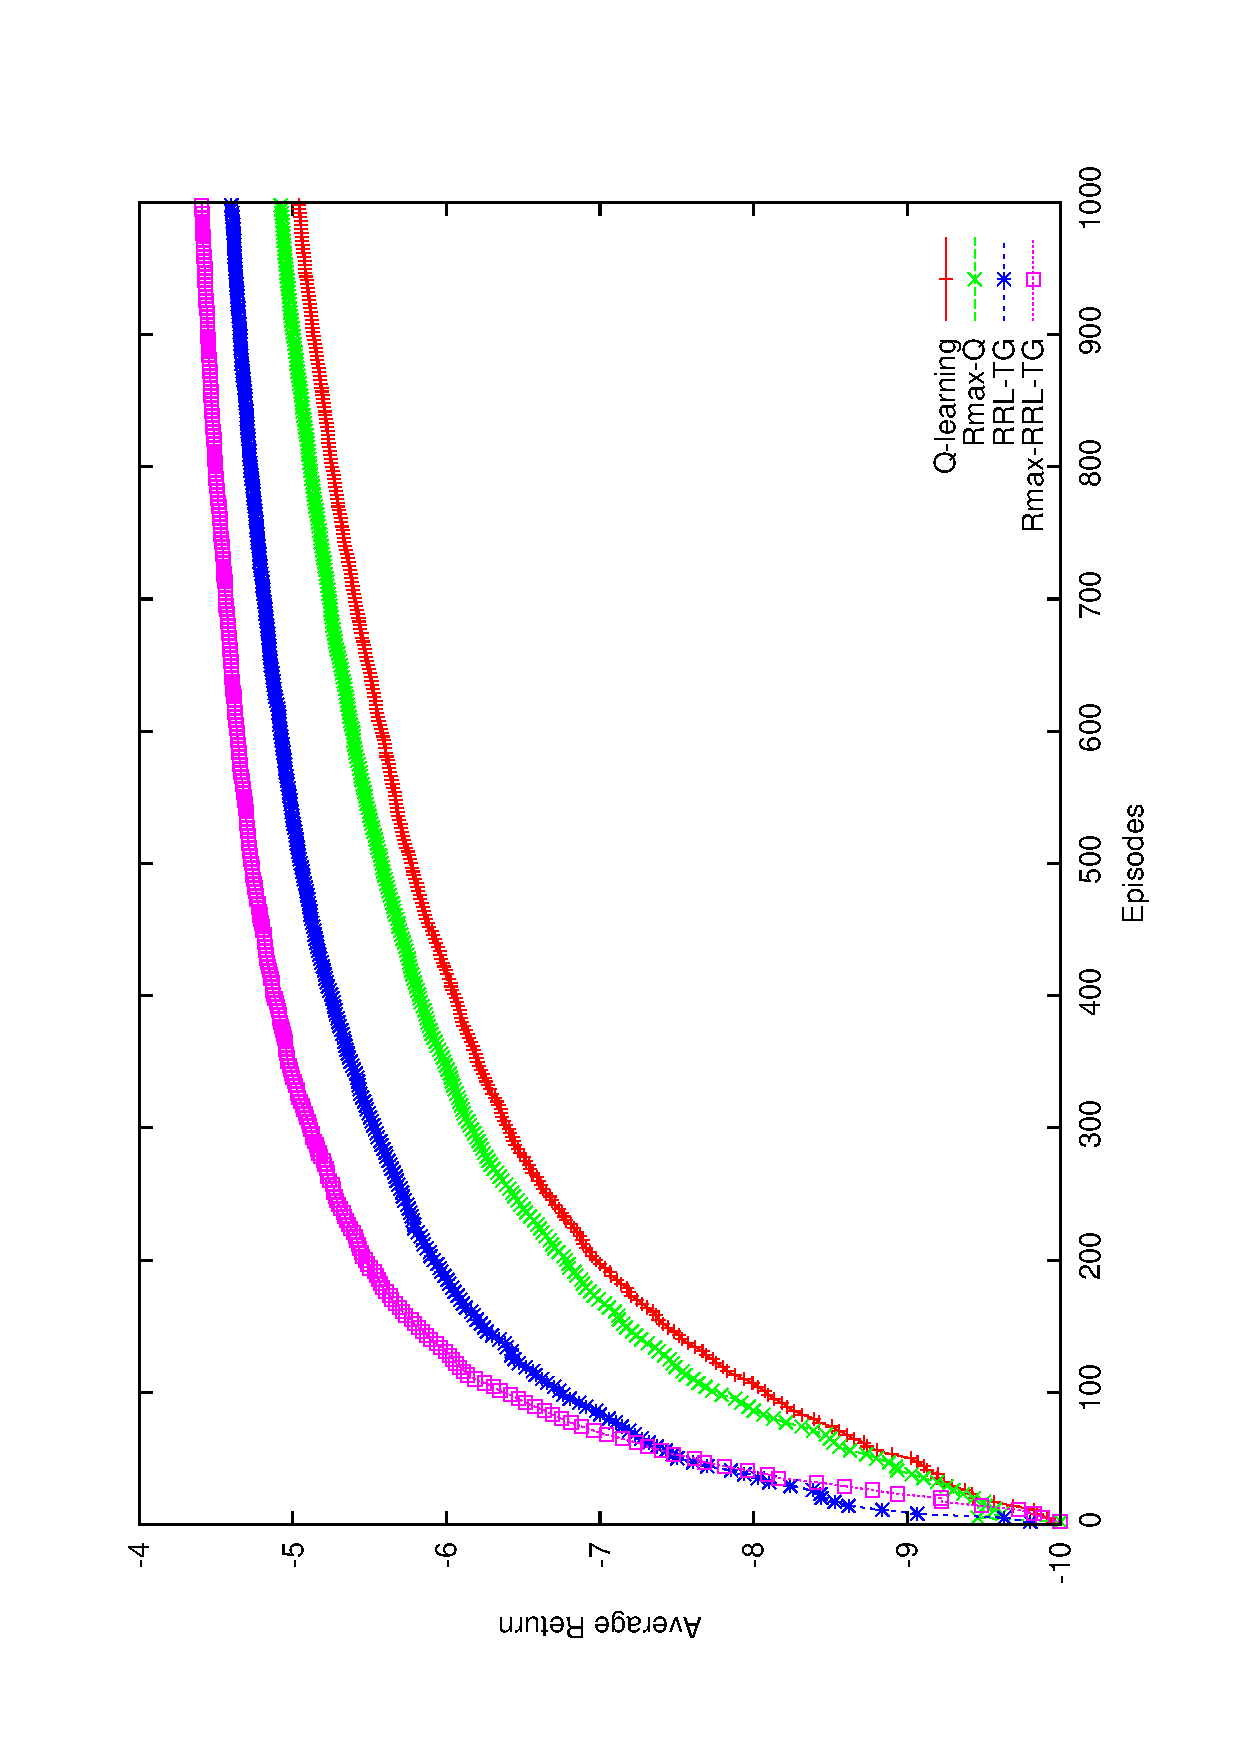
\includegraphics[width=1\columnwidth]{figure1.png}
\caption{The environment is 4 blocks on 3 stacks. The target is putting all the
blocks on the same stack and ordered. Each data point is run for 10 times.}
\label{fig:exp1}
\end{figure}

\begin{figure}
\centering
\includegraphics[width=1\columnwidth]{figure2.png}
\caption{The environment is 3 blocks on 3 stacks. The target is putting all the
blocks on the same stack and ordered. Each data point is run for 10 times.}
\label{fig:exp2}
\end{figure}

The results are shown in Figure~\ref{fig:exp1} and Figure~\ref{fig:exp2}.
The environment of Figure~\ref{fig:exp2} has a smaller state space. Rmax-TG-RRL
does not have as good performance as TG-RRL.

%=============================================================================
\section{Discussion}

The improvement of Rmax-RRL-TG can also be related with hierarchical learning.
When it finds the predicate at the root, it transfers the learning tasks into
its children. This speeds up the learning process.

In Figure~\ref{fig:exp1}, Rmax-RRL-TG shows worse performance than RRL-TG at the
very beginning, because it's not acting optimally. It catches up after
exploration. It also has a similar performance with Q-learning at the beginning.
This is because when the Q-tree is being built, its control is inconsistent with
its knowledge. If a state $s$ has legal actions $a_1$ and $a_2$. $Q(s, a_1) >
Q(s, a_2)$ is known. Q-learning will select $a_1$, if not exploring (with
probability of $\epsilon$). Rmax-RRL-TG might not be able to make this action,
as its Q-tree is not expressive enough to distinguish $a_1$ and $a_2$. However,
considering the advantage of value approximation, model approximation and the
features of hierachical learning, this sacrifice at the beginning is worthy.

This combines algorithms from two domains, but it just applies into relational
RL problems. Blocks world is widely used to show the performance of RRL
algorithms, as it inherently can be expressed as predicates. Many practical
problems might not even be represented in tranditioanl states in RL. It's not
clear wether they can be represented in predicates.

%=============================================================================
\bibliographystyle{named}

\bibliography{report}

\end{document}
